% Generated by code/ch01_hardware.py -- do not edit by hand.
\definecolor{qocA}{rgb}{0.00,0.45,0.70}
\definecolor{qocB}{rgb}{0.90,0.60,0.00}
\definecolor{qocC}{rgb}{0.00,0.62,0.45}
\definecolor{qocD}{rgb}{0.80,0.40,0.00}
\definecolor{qocE}{rgb}{0.80,0.60,0.70}
\definecolor{qocF}{rgb}{0.35,0.70,0.90}
\begin{tikzpicture}[x=1cm,y=1cm]

% background: the cryostat
\node[anchor=south west, inner sep=0] (cryo) at (0,0) {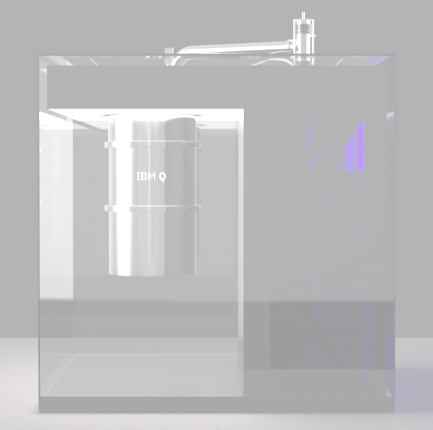
\includegraphics[width=8.00cm]{figures/hw_cryostat.png}};
% wiring stages, seen inside the can (left-centre of the photograph)
\node[anchor=center, inner sep=0, draw=white, line width=0.6pt] (wires) at (2.40,5.04) {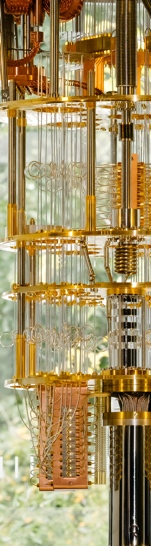
\includegraphics[height=2.72cm]{figures/hw_wires.jpg}};
% zoom 1: the printed circuit board at the bottom of the cryostat
\node[anchor=center, inner sep=0, draw=qocB, line width=1pt] (pcb) at (2.72,2.08) {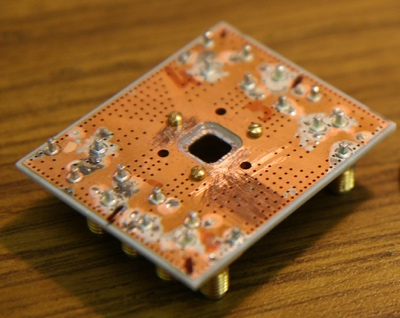
\includegraphics[width=3.20cm]{figures/hw_board.jpg}};
% zoom 2: the qubit chip at the centre of the board
\node[anchor=center, inner sep=0, draw=qocA, line width=1pt] (chip) at (pcb.center) {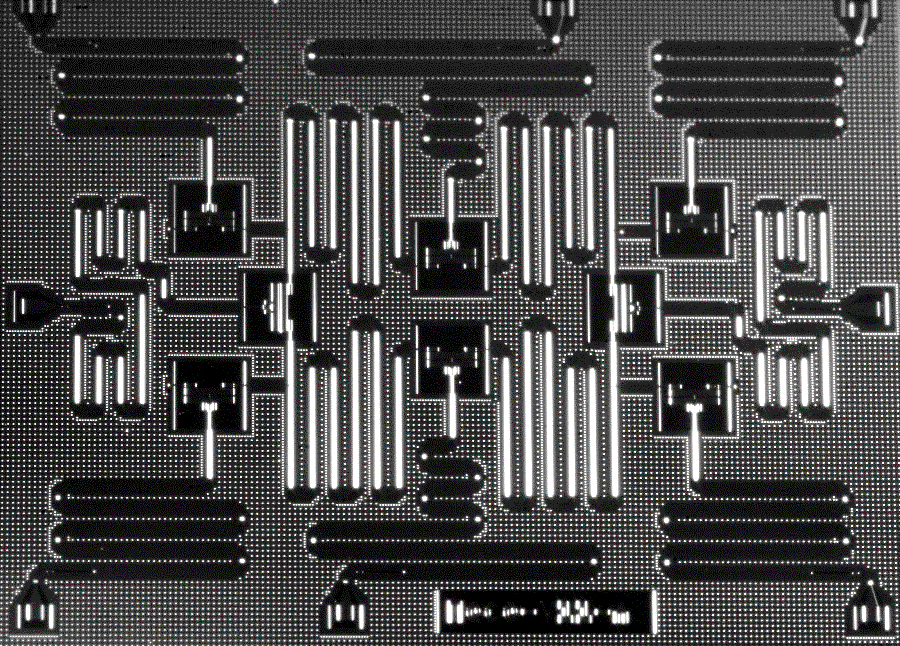
\includegraphics[width=1.36cm]{figures/hw_chip.png}};
% zoom lines
\draw[qocB, thick, dashed] (wires.south west) -- (pcb.north west);
\draw[qocB, thick, dashed] (wires.south east) -- (pcb.north east);
\draw[qocA, thick, dashed] ($(pcb.center)+(-0.12,-0.10)$) -- (chip.south west);
\draw[qocA, thick, dashed] ($(pcb.center)+(0.12,-0.10)$) -- (chip.south east);
% room-temperature electronics, placed over the right half of the cabinet
\node[anchor=south, inner sep=0, draw=white, line width=0.6pt] (rack) at (6.08,2.40) {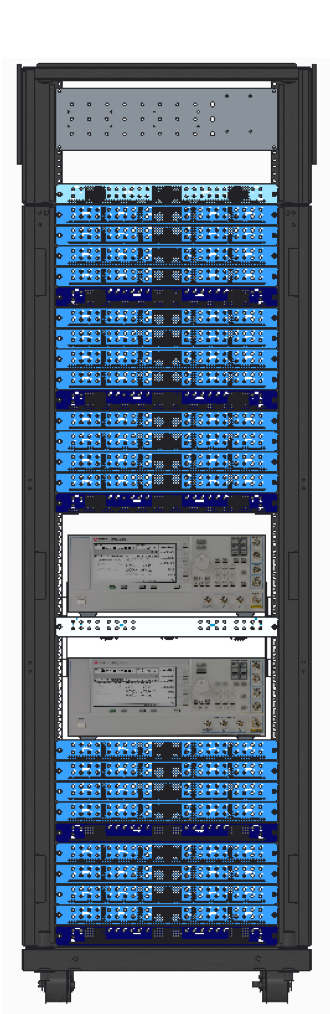
\includegraphics[height=4.80cm]{figures/hw_electronics.png}};
% labels
\small
\node[anchor=north west, align=left, font=\small\bfseries, fill=white, fill opacity=0.8, text opacity=1, inner sep=1.5pt] at (0.05,7.95) {dilution cryostat (Bluefors),\\ about 10\,mK};
\node[anchor=west, align=left, fill=white, fill opacity=0.8, text opacity=1, inner sep=1pt, font=\footnotesize] at ($(wires.east)+(0.06,0.5)$) {wiring and\\ filtering stages\\ (fragile below 1\,K)};
\node[anchor=north, align=center, fill=white, fill opacity=0.8, text opacity=1, inner sep=1pt, text=qocB] at ($(pcb.south)+(0,-0.05)$) {circuit board (zoom)};
\node[anchor=south, align=center, fill=white, fill opacity=0.8, text opacity=1, inner sep=1pt, text=qocA] at ($(chip.north)+(0,0.03)$) {qubit chip (zoom)};
\node[anchor=north, align=center, font=\small, text width=2.88cm, fill=white, fill opacity=0.85, text opacity=1, inner sep=2pt] at ($(rack.south)+(0,-0.08)$) {room-temperature electronics: signal sources, FPGA pulse shaping, digitisers -- \alert{this is where $u(t)$ is made}};
\node[anchor=north east, font=\tiny, fill=white, fill opacity=0.8, text opacity=1, inner sep=1pt] at (8.00-0.05,7.95) {Image credit: IBM.};
\end{tikzpicture}
